% ----------------------------------------------------------------------
\renewcommand{\CurrentProgressBarIs}{\OneOfFive}
% ----------------------------------------------------------------------
\begingroup
% \setbeamercolor{normal text}{bg=black}
\setbeamercolor{background canvas}{bg=mLightBrown!10}
\begin{frame}[t,plain]{1. Introduction}
\end{frame}
\endgroup
% ----------------------------------------------------------------------
\begin{frame}[t]{Introduction: Motivation}

\centering

% \vspace*{-4mm}
\vspace*{-2mm}

\begin{tikzpicture}
\draw (0, 0) node[inner sep=0] {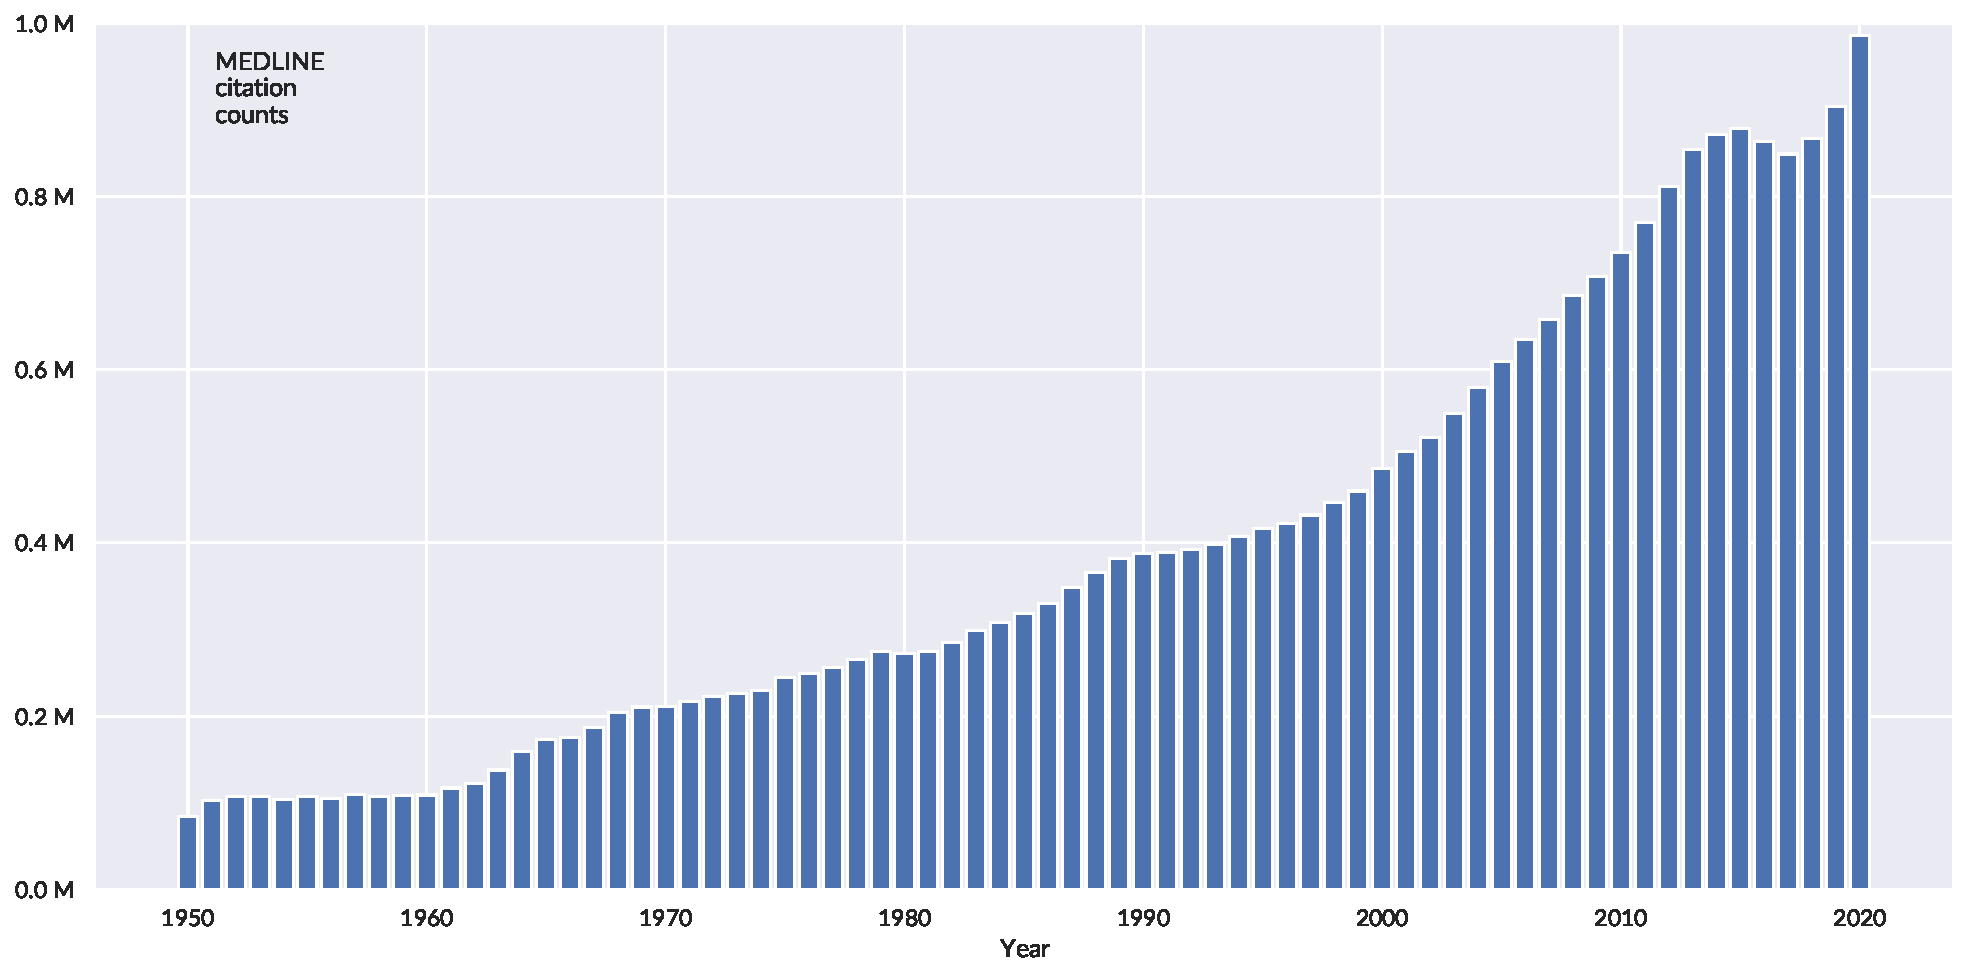
\includegraphics[width=\textwidth]{img/medline/v2/img.pdf}};

\node[anchor=west] at (-5.45, 1.70) {\large\textbf{\alert{How to connect the existing knowledge}}};
\node[anchor=west] at (-5.45, 1.15) {\large\textbf{\alert{by automatic means?}}};

\end{tikzpicture}

\vspace*{-1mm}

\fontsize{5pt}{6pt}\selectfont
Source:
\url{https://www.nlm.nih.gov/bsd/medline_cit_counts_yr_pub.html}
% (accessed September 19, 2021)

\end{frame}
% ----------------------------------------------------------------------
\begin{frame}[t]{Introduction: Biomedical text mining}

\centering

% \vspace*{-4mm}
% \vspace*{-2mm}
\vspace*{10mm}

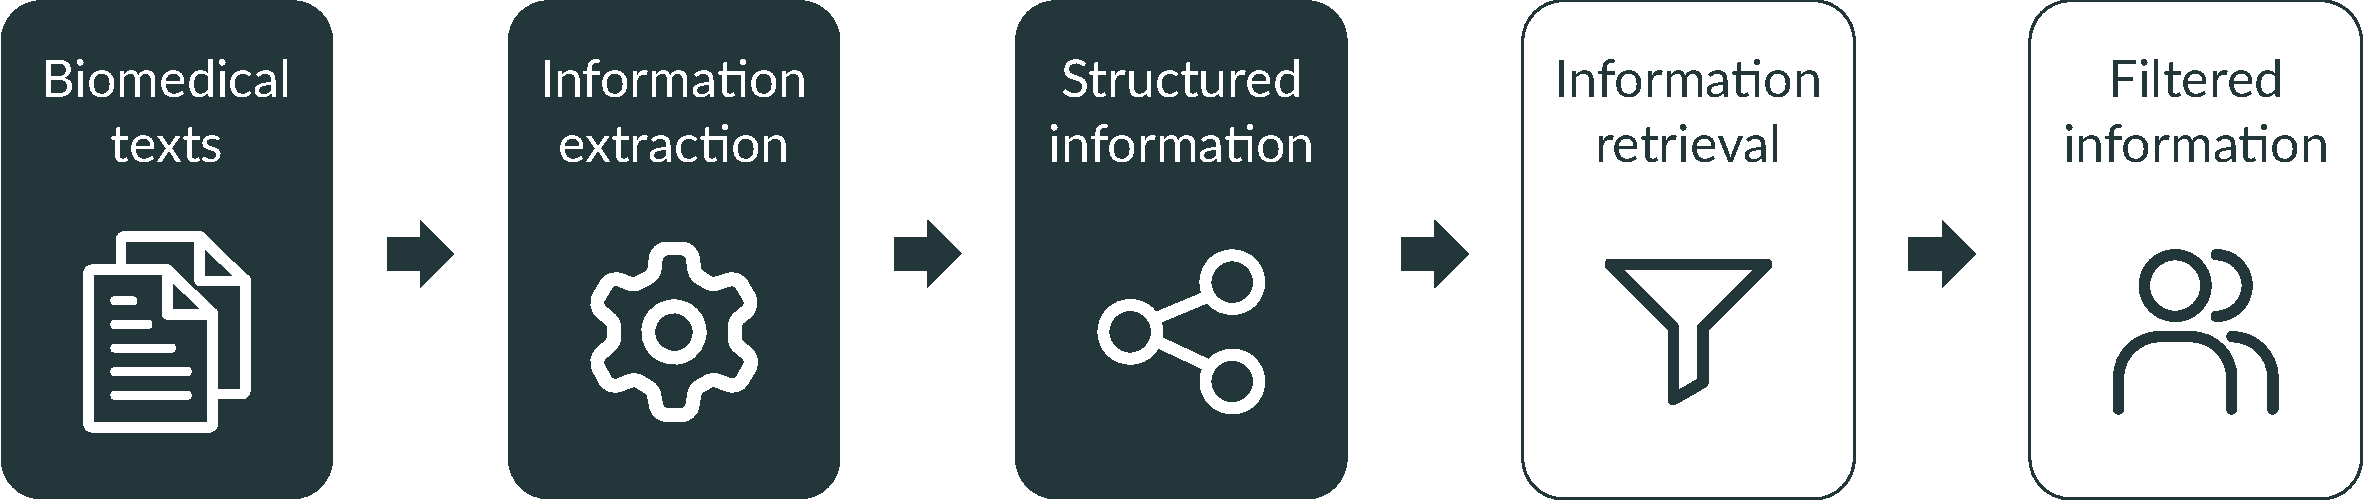
\includegraphics[width=\textwidth]{img/biomedical-text-mining/v1/004.pdf}%

\end{frame}
% ----------------------------------------------------------------------
\begingroup
% \linespread{1.6}
\linespread{2.0}

\renewcommand{\reducedstrut}{\vrule width 0pt height .6\ht\strutbox depth .6\dp\strutbox\relax}

\renewcommand{\cb}[2]{%
\setlength{\fboxsep}{2pt}%
\colorbox{#1}{\reducedstrut#2}%
}

\begin{frame}[t]{Introduction: Research challenge}

% \centering

% \scriptsize % 8pt
% \fontsize{7.25pt}{8.7pt}\selectfont
% \fontsize{7.0pt}{8.4pt}\selectfont
\fontsize{6.5pt}{7.8pt}\selectfont
% \tiny % 6pt
\begin{justify}
A patient with rheumatoid arthritis developed an acute \cb{red!20}{intrahepatic cholestasis} after \cb{green!20}{100 mg} of \cb{blue!20}{sodium aurothiomalate}. Hepatotoxicity in rheumatoid arthritis is well described following a variety of anti-inflammatory preparations but is now a rare complication of gold therapy and the literature on the subject is reviewed.
\end{justify}

\vspace*{8mm}
% \bigskip\smallskip
% \bigskip

% Sources:
%   Entities:
%     https://uts.nlm.nih.gov/uts/umls/concept/C0008372
%     https://uts.nlm.nih.gov/uts/umls/concept/C0018034
%   Relations:
%     https://uts.nlm.nih.gov/uts/umls/concept/C0413732
%     https://uts.nlm.nih.gov/uts/umls/concept/C0357546

\begin{tabular}{@{}l@{\hskip40pt}l@{}}

\cb{red!20}{intrahepatic cholestasis} \cb{orange!20}{C0008372} & \cb{blue!20}{sodium aurothiomalate} $\xrightarrow[\textnormal{\fontsize{5.0pt}{6.0pt}\selectfont\cb{orange!20}{C0413732}}]{\textnormal{\fontsize{6.5pt}{7.8pt}\selectfont~~~~~~~~~~~~Drug adverse effect~~~~~~~~~~~~}}$ \cb{red!20}{intrahepatic cholestasis}\\[24pt]

\cb{blue!20}{sodium aurothiomalate} \cb{orange!20}{C0018034} & \cb{blue!20}{sodium aurothiomalate} $\xrightarrow[\textnormal{\fontsize{5.0pt}{6.0pt}\selectfont\cb{orange!20}{C0357546}}]{\textnormal{\fontsize{6.5pt}{7.8pt}\selectfont~~~~~~~~~~~~Drug dosage~~~~~~~~~~~~}}$ \cb{green!20}{100 mg}

\end{tabular}

\vspace*{7mm}

\flushleft
\fontsize{5pt}{6pt}\selectfont
Source: ADE corpus (PMID 115078)

\end{frame}
\endgroup
% ----------------------------------------------------------------------
\begin{frame}[t]{Introduction: Biomedical information extraction}

\centering

% \vspace*{-4mm}
% \vspace*{-2mm}
% \vspace*{10mm}

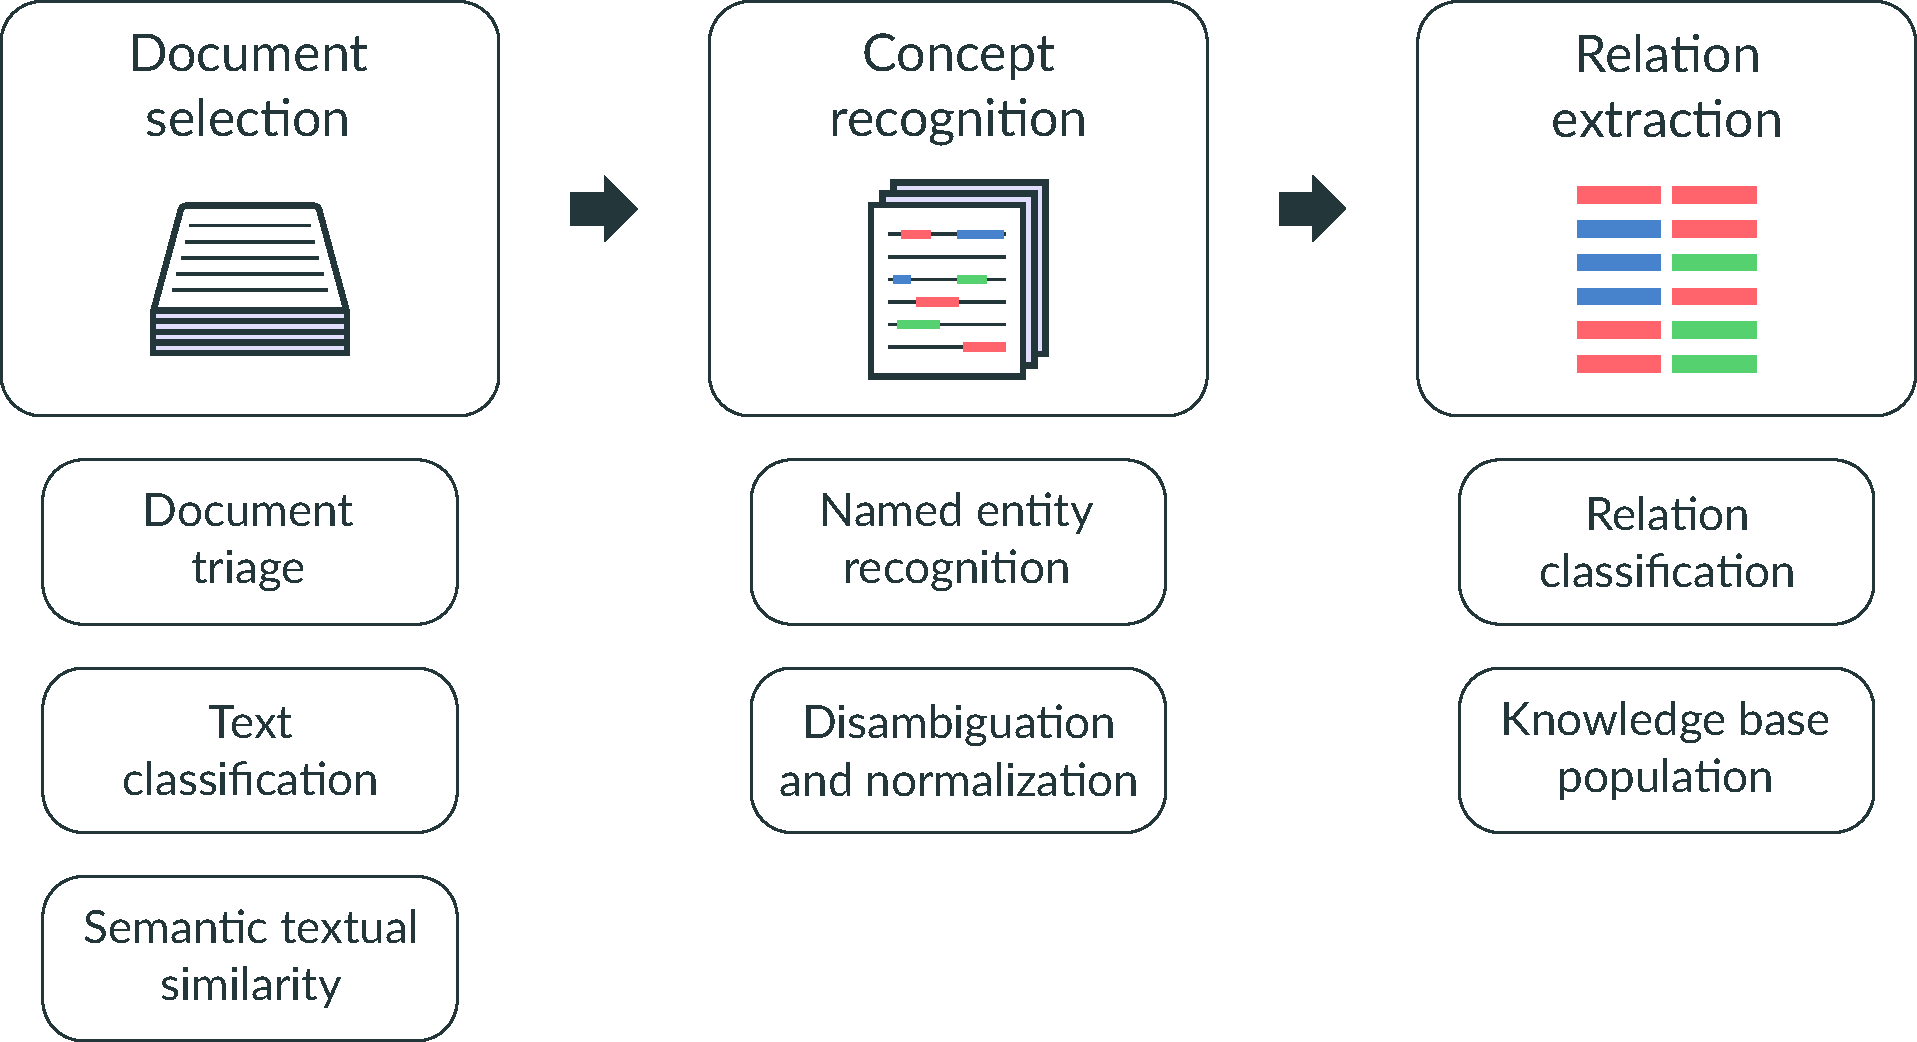
\includegraphics[width=0.80\textwidth]{img/biomedical-information-extraction/v3/003.pdf}%

\end{frame}
% ----------------------------------------------------------------------
\begin{frame}[t]{Introduction: Text encoding}

% \centering

% \vspace*{-4mm}
% \vspace*{-3mm}
% \vspace*{-2mm}
% \vspace*{4mm}
% \vspace*{10mm}

\small
\textbf{Sparse representation}

\vspace*{-0.4\topsep}
\begin{itemize}
\setlength{\itemsep}{0.0pt}
\item One-hot encoding
\item Term frequency--inverse document frequency (TF--IDF)
\end{itemize}

\vspace*{4mm}
% \vspace*{8mm}

\textbf{Dense representation}

\vspace*{-0.4\topsep}
\begin{itemize}
\setlength{\itemsep}{0.0pt}
\item Word embeddings (distributed representations of words)
\end{itemize}

% \vspace*{1mm}

\begingroup\setlength{\leftmargini}{14mm}%
\tiny%
\blockquote{\textit{Mikolov et al. introduced the Skip-gram model, \alert{an efficient method for learning high-quality vector representations of words from large amounts of unstructured text data}. Unlike most of the previously used neural network architectures for learning word vectors, training of the Skip-gram model does not involve dense matrix multiplications. This makes the training extremely efficient: \alert{an optimized single-machine implementation can train on more than 100~billion words in one day}.}}%

\vspace*{2mm}

\fontsize{5pt}{6pt}\selectfont%
\begin{tabular}{@{\hskip\leftmargini}l@{\hskip2pt}l}
Source: & Tomas Mikolov, Ilya Sutskever, Kai Chen, Greg Corrado, and Jeffrey Dean (December 2013).\\%
& \textit{Distributed representations of words and phrases and their compositionality}. NIPS 2013.
\end{tabular}

\endgroup

% Sources:
% https://arxiv.org/abs/1301.3781
% https://arxiv.org/abs/1310.4546

\end{frame}
% ----------------------------------------------------------------------
\begin{frame}[t]{Introduction: Word embeddings example}

\centering

\vspace*{-4mm}
% \vspace*{-2mm}

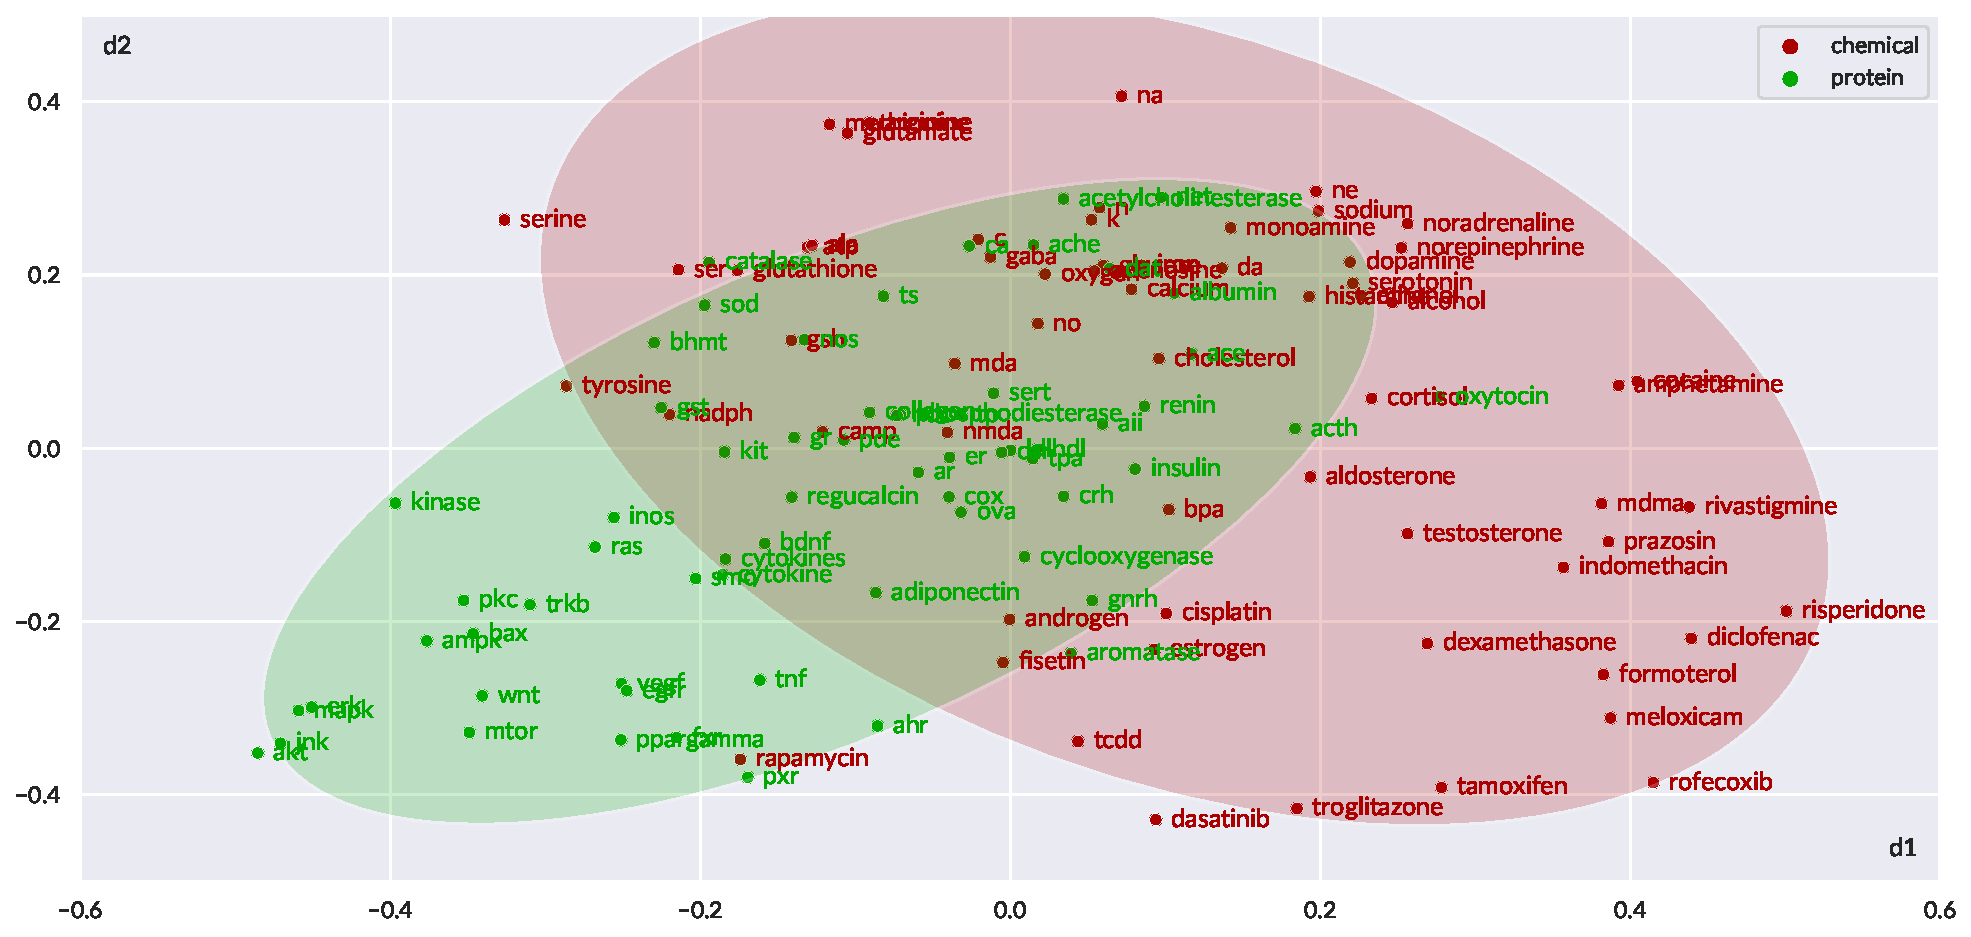
\includegraphics[width=\textwidth]{img/chemprot-word-embeddings/v2/128-ellipses.pdf}%

\vspace*{1mm}

\fontsize{5pt}{6pt}\selectfont
Embeddings calculated using the BioWordVec model for entities in the ChemProt corpus

\end{frame}
% ----------------------------------------------------------------------
\begin{frame}[t]{Introduction: Word embeddings example}

% \centering

% \vspace*{-4mm}
% \vspace*{-2mm}
\vspace*{2mm}

% Considering the expression:
\begingroup\large
\textit{yellow fever viral disease} $\rightarrow$ \texttt{['yellow', 'fever', 'viral', 'disease']}
\endgroup

\vspace*{6mm}

% Add invisible hyphens (to align the vectors).
% https://tex.stackexchange.com/questions/4519/how-do-i-create-an-invisible-character
\begin{center}
\renewcommand*{\arraystretch}{1.2}
\begin{tabular}{cc}
% \toprule
Word & Vector\\
\midrule
\texttt{'yellow'}  & \texttt{\small [ -0.163,  \phantom{-}0.027, ..., \phantom{-}0.009 ]}\\
\texttt{'fever'}   & \texttt{\small [ \phantom{-}0.037,  -0.169, ..., \phantom{-}0.062 ]}\\
\texttt{'viral'}   & \texttt{\small [ -0.037,  -0.115, ..., \phantom{-}0.056 ]}\\
\texttt{'disease'} & \texttt{\small [ \phantom{-}0.141,  -0.107, ..., -0.031 ]}\\
\midrule
Average vector & \texttt{\small [ -0.006,  -0.091, ..., \phantom{-}0.024 ]}\\
% \bottomrule
\end{tabular}
\end{center}

\end{frame}
% ----------------------------------------------------------------------
